\chapter{実数の連続性と極限}
\label{chp:realnumber}
 この章では,Dedekindによる切断と呼ばれる概念を用いて
 有理数をもとにして実数の公理系を満たすモデルを構成し,
 実数の連続性,および極限について考察する.

 実数や極限に関しては高校で学んでいるが,
 その議論は直感に訴えたものであった.
 この章では,実数や極限に関する
 基本的な性質をあいまいさ抜きに
 探っていくことを第一の目標とする.

 また,この章ではCauchyの試みが生み出した$\varepsilon$-$N$論法
 と呼ばれる論法が登場する.
 この論法は「限りなく大きくなる」や「限りなく近づく」という概念を
 「すべて」や「存在」を巧みに使って定式化した論法である.
 学び始めてしばらくは戸惑いを覚えるかもしれないが,
 慣れてしまえば少しも難しくないことに気がつくはずである.
 
 この章の内容は微分積分学の入門的な内容と重複する部分が多い.
 読者は微分積分学を学んだあとに,あるいは微分積分学と並行して
 この章を読み進めるとよい.

 
%
 \section{\textrm{Dedekind}切断による実数の構成}
 \label{sec:dedekind}
   この節では,有理数とその性質は既知として,そこから実数を構成することを考える.
 
   \paragraph{有理数の切断}
   有理数全体の集合$\mathbb{Q}$を次の(a$),($b$),($c)の条件を満たす
    $A,  B$の2つの部分集合に分割する.この$A,  B$
    の組を
    \index[widx]{ゆうりすう@有理数 \, rational number!
    ゆうりすうのせつだん@---の切断 \, cut of ---s}
    \emph{有理数の切断}(cut of rational numbers)といい,
    $(A \mid B)$と表す.
    \begin{enumerate}[(a) ]
      \item $A \neq \varnothing ,  B \neq \varnothing ,  
        A \cup B = \mathbb{Q} ,  A \cap B = \varnothing .$
      \item $\forall a \in A \forall b \in B ( a<b) .$
      \item $A$には最大数がない.
    \end{enumerate}
    有理数の切断$(A \mid B)$には,$B$に最小数が存在するものと
    $B$に最小数が存在しないものの2種類が考えられる.

    \begin{figure}[h]
      \centering
      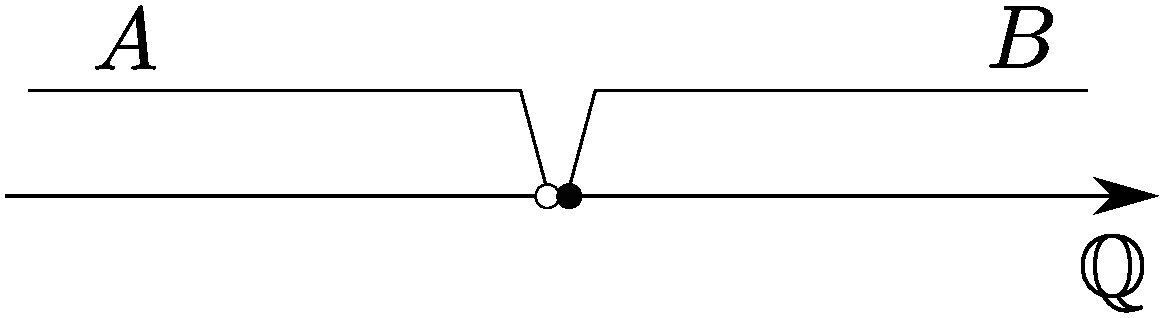
\includegraphics[width=4.7cm]{inputyou/realnumber/picture/cutrational1.pdf}
      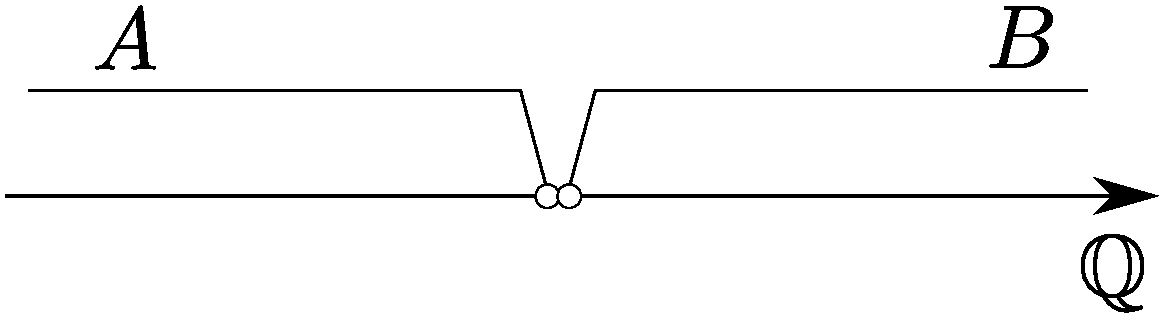
\includegraphics[width=4.7cm]{inputyou/realnumber/picture/cutrational2.pdf}
      \caption{有理数の切断} \label{fig:cutrational}
    \end{figure}

    \begin{ex} \label{ex:cutrational}
      有理数$r$を1つとり,集合$A_r,  B_r$を
      \begin{align*}
        A_r & = \Set{ x \in \mathbb{Q} \mid x < r} , \\
        B_r & = \Set{ x \in \mathbb{Q} \mid x \geq r}
      \end{align*}
      と定めると,$(A_r \mid B_r)$は有理数の切断である.
      また,$r \in B$が$B$の最小数である.
    \end{ex}

    \begin{ex} \label{ex:cutrational2}
      よく知られているように,$r^2=2$を満たす有理数$r$は存在しない.
      集合$A,  B$を
      \begin{align*}
        A & = \Set{ r \in \mathbb{Q} \mid r < 0 \lor r^2 <2 } , \\
        B & = \Set{ r \in \mathbb{Q} \mid r>0 \land r^2>2 }
      \end{align*}
      と定める.
    
      $A,B$が条件(a$),($b)を満たすことは明らかであろう.
      $A$には最大数が存在しないことを示そう.
      $a>0$を満たす$a \in A$を任意にとると,
      $a^2<2$である.そこで,
      \[
        h = \frac{1}{2} \min \Set{ \frac{2-a^2}{2a+1} ,  1}
      \]
      とおくと,$h$は
      \[ 
        0<h<1 , h < \frac{2-a^2}{2a+1}
      \]
      を満たす.$x=a+h$とおくと$x>a$であり,さらに
      \begin{align*}
        x^2 & = (a+h)^2 \\
            & = a^2 +2ah + h^2 \\
            & < a^2 + (2a + 1)h \\
            & < a^2 + (2a+1) \cdot \frac{2-a^2}{2a+1} \\
            & = 2
      \end{align*}
      だから$x \in A$である.
      従って,$A$には最大数が存在しない.
      同様にして$B$に最小数が存在しないことも導ける.
    \end{ex}

    例\ref{ex:cutrational2}からもわかるように,
    有理数の範囲で考えると,切断の「境界」にあたる数が
    存在しないことがある.
    そこで,
    その境界にあたる数を新たに付け加えて数の体系を拡張したいのだが,
    この「境界にあたる数」を具体的な形で定義したいというのが
    我々の目的であった.
    そこで,有理数の切断さえ与えてしまえばその「境界」は一意に確定する
    \footnote{我々が有理数の切断に条件(c)を課した意義がここにある.}
    ことに着目して,有理数の切断そのものを数だとみなし,
    \begin{align}
      \mathbb{R} = \Set{ (A \mid B) \mid (A \mid B) \text{は有理数の切断である}}
      \label{eq:realnumber}
    \end{align}
    と定め,$\mathbb{R}$の元を
    \index[widx]{じっすう@実数 \, real number}
    \emph{実数}(real number)と呼ぶことにする.

   \paragraph{埋め込み}
    $r \in \mathbb{Q}$に対し,例\ref{ex:cutrational}で定義された
    有理数の切断$(A_r \mid B_r)$を対応させる写像を$\iota : \mathbb{Q} \longrightarrow \mathbb{R}$
    とおくと,$\iota$は単射である.
    この写像$\iota$を$\mathbb{Q}$の$\mathbb{R}$への
    \index[widx]{うめこみ@埋め込み \, embedding}
    \emph{埋め込み}(embedding)という.

    有理数$r$について考えるのと$\iota (r) = ( A_r \mid B_r)$
    について考えるのは「同じこと」である
    \footnote{しかし,何がどう「同じ」なのかはこの段階ではまだわからない.
    このことは$\mathbb{R}$に順序や演算を導入して初めてわかることである.}
    .
    そこで,有理数$r$と$r$に対応する有理数の切断$\iota (r) = (A_r \mid B_r)$
    を同一視して,$\mathbb{Q} \subset \mathbb{R}$とみなすことにする.
    すなわち,$\iota (\mathbb{Q} )$をそのまま$\mathbb{Q}$とみなす.
    $\mathbb{R}$の元のうち,$\iota (\mathbb{Q})$
    の元でもあるものを
    \index[widx]{ゆうりすう@有理数 \, raional number}
    \emph{有理数}(rational number)といい,
    そうでないものを
    \index[widx]{むりすう@無理数 \, irrational number}
    \emph{無理数}(irrational number)という.
    たとえば,例\ref{ex:cutrational2}で考えた有理数の切断は,
    通常$\sqrt{2}$と表される無理数である.

   \paragraph{実数の大小}
    $\alpha,  \beta \in \mathbb{R}$に対し,$\alpha$と$\beta$を定義する
    2つの有理数の切断$\alpha=(A \mid B) ,  \beta=(C \mid D)$をとる.
    集合$A,  C$が$A \subset C$を満たすとき,
    $\alpha \leq \beta $あるいは$\beta \geq \alpha$と表す.
    集合$A,  C$が$A=C$を満たすとき,
    $\alpha = \beta$であるとする.さらに,$\alpha \leq \beta$かつ$\alpha \neq \beta$であることを
    $\alpha < \beta$あるいは$\beta > \alpha$と表す.
    $\alpha < \beta$であることは$A \subsetneq C$であること
    に相当する.

    明らかに,有理数の切断が有理数を表す場合には,
    以上のように定義した実数の大小の定義ともとの有理数の大小は矛盾しない.

    \begin{lemma} \label{lemma:daisyouwelldefined}
      任意の$\alpha ,  \beta \in \mathbb{R}$に対し,
      $\alpha=\beta,  \alpha<\beta,  \alpha>\beta$
      のうちのどれか1つだけが必ず成立する.
    \end{lemma}

    \begin{proof}
      $\alpha = \beta$の場合,実数の大小の定義から$\alpha < \beta$も$\alpha > \beta$
      も成り立たない.そこで,$\alpha \neq \beta$の場合を考える.
      いま,有理数の切断によって$\alpha = (A \mid B) ,  \beta = (C \mid D)$
      と表すと,$\alpha \neq \beta$であるから$A \neq C$である.
      よって,$A$か$C$のどちらか一方にのみ属する有理数$r$が存在する.
      $r \in A$かつ$r \notin C$とすると,$r \in D$であり,
      任意の$c \in C$に対して$c < r$となり,$r \in A$だから$c \in A$であり,
      $C \subsetneq A$が成り立つ.よって$\alpha > \beta$である.
      $r \in C$かつ$r \notin A$の場合も同様にして$\alpha < \beta$となる.
      真部分集合の定義により,$\alpha < \beta$と$\alpha > \beta$
      が同時には成り立たないことは明らかであろう.
    \end{proof}


    次の定理\ref{thm:realdaisyou}は,集合の包含関係の性質から明らかである.
    \begin{thm} \label{thm:realdaisyou}
      実数の大小関係は,
      \begin{align}
        \forall \alpha \in \mathbb{R} (\alpha \leq \alpha) ,
        \label{eq:realreflexive} \\
        \forall \alpha , \beta \in \mathbb{R} 
        ( \alpha \leq \beta \land \beta \leq \alpha \to \alpha = \beta) ,
        \label{eq:realsymmetry} \\
        \forall \alpha , \beta ,\gamma \in \mathbb{R} 
        ( \alpha \leq \beta \land \beta \leq \gamma \to \alpha \leq \gamma)
        \label{eq:realsuiiritu}
      \end{align}
      を満たす.
    \end{thm}

    次の補題\ref{lemma:cutdaisyou}は直感的には明らかであるが,
    定義に従って証明しておこう.
    \begin{lemma} \label{lemma:cutdaisyou}
      実数$\alpha$を有理数の切断により$\alpha = (A \mid B)$と表したとき,
      \[
        \forall a \in A \forall b \in B( a < \alpha \leq b)
      \]
      が成り立つ.
    \end{lemma}

    \begin{proof}
      $a \in A,   b \in B$を任意にとり,
      有理数の切断によって$a = (C \mid D) ,  b= (E \mid F)$と表す.
      $c \in C$を任意にとると,$a$が有理数であることから$a$は$D$の最小数であり,
      従って$c <a$となる.よって$c \in A$となり,$C \subset A$となる.
      ゆえに$a \leq \alpha$となる.
      また,$A$に最大数が存在しないことから,$a<m$となる$m \in A$がとれる.
      同様にして$m \leq \alpha$が成り立つので,$a<m \leq \alpha$より
      $a< \alpha $となる.
      また,$u \in A$を任意にとると,$(A \mid B)$が有理数の切断であることから
      $b \in B$より$a<b$となる.$b$は有理数であるから$b$は
      $F$の最小数であり,$u \in E$となる.
      よって$A \subset E$となり,$\alpha \leq b$がいえ,
      $a < \alpha \leq b$を得る.
    \end{proof}

    \index[widx]{ゆうりすう@有理数 \, rational number!
    ゆうりすうのちゅうみつせい@---の稠密性 \, density of the ---s}
    \begin{thm}[有理数の\ruby{稠密性}{ちゅうみつせい}] \label{thm:yurisutyumitu}
      $\alpha < \beta $を満たす任意の実数$\alpha ,  \beta$に対し,
      $\alpha <r< \beta$を満たす有理数$r$が少なくとも1つ,
      従って無限に多く存在する.
    \end{thm}
    \begin{proof}
      有理数の切断により,$\alpha = (A \mid B) ,  \beta = (C \mid D)$と表す.
      $\alpha < \beta$であるから$A \subsetneq C$であり,
      $q \notin A$かつ$q \in C$を満たす有理数$q$が存在する.
      $C$には最大数が存在しないので,
      $q < r$を満たす$r \in C$がとれる.
      すると,$r < \beta$が成り立つ.
      また,$q \notin A$より$q \in B$であるから$r \in B$であり,
      $\alpha \leq q<r$,すなわち$\alpha < r $を得る.
      従って$\alpha < r < \beta$である.
      この$r$はもちろん実数であるから,同様にして$\alpha < r_1<r$を満たす
      有理数$r_1$をとることができる.
      以上の議論を繰り返すことにより,$\alpha < r < \beta$を満たす
      有理数$r$はいくらでも多くとれる.
    \end{proof}


   \paragraph{実数の演算}
    ここからは,$\mathbb{R}$に加法や乗法といった演算を導入することを考える.
    \begin{thm} \label{thm:realwawelldef}
      実数$\alpha ,  \beta$を有理数の切断によって
      $\alpha = (A \mid B) ,  \beta = (C \mid D)$
      と表す.このとき,
      \begin{align*}
        E & = \Set{ a+ c \mid a \in A,  c \in C} , \\
        F & = \mathbb{Q} - E
      \end{align*}
      とおくと,組$(E \mid F)$は有理数の切断である.
      この切断$(E \mid F)$を$\alpha ,  \beta$の
      \index[widx]{じっすう@実数 \, real number!じっすうのわ@---の和 \, sum of ---s}
      \emph{和}(sum)といい,$\alpha + \beta$と表す.
    \end{thm}
    \begin{proof}
      明らかに$E \neq \varnothing,  
      E \cup F = \mathbb{Q} ,  E \cap F = \varnothing$である.
      $F \neq \varnothing$を示したい.それには$E \neq \mathbb{Q}$を示せばよい.
      $ B,   D$は空でないので$b \in B$と$d \in D$がとれる.
      任意の$a \in A,  c \in C$に対して$a<b$かつ$c<d$であるから
      $a+c<b+d$である.従って,有理数$b+d$は$a \in A ,  c \in C$
      の和の形には表されない.よって$b+d \notin E$であり,$E \neq \mathbb{Q}$
      となる.

      次に,$\forall e \in E \forall f \in F(e<f)$を示したい.
      それには任意の$e \in E$に対し,$r<e$を満たす任意の有理数$r$が
      $r \in E$を満たすことを示せばよい.
      $e \in E$だから,$a+c = e$となる$a \in A,  c \in C$がとれる.
      $q = c-( e-r)$とおくと$e-r>0$より$q<c$であり,$c \in C$だから$q \in C$
      となる.従って,$r=a+q$は$a \in A$と$q \in C$の和の形で表せる.
      よって$r \in E$.
      
      最後に$E$に最大数がないことを示せば証明は完結する.
      $e \in E$を任意にとると,$e= a+c$となる$a \in A,  c \in C $
      が存在する.$A,  C$はともに最大数をもたないので,
      $a < u ,  c<v$となる$u \in A ,  v \in C$をとることができる.
      $x=u+v$とおくと,$x \in E$であり$e<x$を満たす.
      ゆえに$E$には最大数はない.
    \end{proof}

    有理数のときに成り立っていた加法に関する種々の性質は,
    実数においても成り立つ.証明は容易であろう.
    \begin{thm} \label{thm:realsumseisitu}
      実数の加法は次の性質を満たす.
      \begin{align}
        \forall \alpha , \beta \in \mathbb{R} ( \alpha + \beta = \beta + \alpha),
        \label{eq:realsumkoukan} \\
        \forall \alpha , \beta , \gamma \in \mathbb{R}
        ((\alpha + \beta ) + \gamma = \alpha + ( \beta + \gamma)). 
        \label{eq:realsumketugou} 
      \end{align}
    \end{thm}
    \begin{que} \label{que:sumunitele}
      任意の実数$\alpha$に対し$\alpha + 0 = \alpha$が成り立つことを示せ.
    \end{que}

    \begin{lemma} \label{lemma:realQkinji}
      実数$\alpha$と正の有理数$r$に対し,
      $a< \alpha < b$かつ$b-a=r$となる有理数$a,  b$が存在する.
    \end{lemma}
    \begin{proof}
      $\alpha$を有理数の切断によって$\alpha = (A \mid B)$と表すと,
      $A \neq \varnothing$より$a_0 \in A$がとれる.
      自然数$n$に対して$a_n=a_0 + nr$とおくと,
      $n$を十分大きくすれば$a_n$の値をいくらでも大きくすることができるから,
      $a_n \in B$となる番号$n$が存在する.
      $a_n \in B$を満たす$n$のうち最小のものをとり,これを$N$とおく.
      $a_N = \alpha$の場合には$b= a_N + r/2$とし,
      そうでない場合には
      $b=a_N$とし,$a= b-r$とおけば
      $a < \alpha <b$と$b-a =r$が成り立つ.
    \end{proof}

    \begin{thm} \label{thm:sumreverse}
      任意の実数$\alpha$に対し,$\alpha + \xi = 0$となる
      実数$\xi$が存在する.
      この$\xi$を$- \alpha$と表す.
    \end{thm}

    \begin{proof}
      有理数の切断により$\alpha = (A \mid B)$と表し,
      \begin{align*}
        C & = \Set{ -b \mid b \in B } , \\
        D & = \Set{ -a \mid a \in A } 
      \end{align*}
      とおくと,組$(C \mid D)$は有理数の切断になる.
      $\xi = (C \mid D)$とおく.$\alpha + \xi =0$
      であることを示したい.いま,有理数の切断により
      $\alpha + \xi  = ( E \mid F),  0=(G \mid H)$と表す.
      $e \in E$を任意にとれば,$e= a-b$となる
      $a \in A$と$b \in B$が存在する.
      $a<b$であるから$e<0$であり,$e \in G$.
      ゆえに$E \subset G$である.
      また,$g \in G$を任意にとると$g <0$だから$-g >0$.
      補題\ref{lemma:realQkinji}により
      $-g=b-a$,すなわち$g=a-b$となる$a \in A,  b \in B$
      が存在する.$g=a+(-b)$で$-b \in C$だから$g \in E.$
      よって$G \subset E$となり$E=G$がいえる.
      従って,$\alpha + \xi =0$である.
    \end{proof}

    実数$\alpha$について,$\alpha >0$が成り立つ場合,
    $\alpha$は
    \index[widx]{じっすう@実数 \, real number!せいのじっすう@正の--- \, positive ---}
    \emph{正}(positive)であるといい,
    $\alpha <0$である場合,$\alpha$は
    \index[widx]{じっすう@実数 \, real number!ふのじっすう@負の--- \, negative}
    \emph{負}(negative)であるという.

    \begin{thm} \label{thm:realproduct}
      2つの正の実数$\alpha ,  \beta$に対し,
      有理数の切断によって$\alpha = (A \mid B) ,  \beta = (C \mid D)$
      と表す.このとき
      \begin{align*}
        F & = \Set{ bd \mid b \in B, d \in D} , \\
        E & = \mathbb{Q} - F
      \end{align*}
      とおくと,組$(E \mid F)$は有理数の切断である.
      この切断$(E \mid F)$を$\alpha ,  \beta$の
      \index[widx]{じっすう@実数 \, real number!じっすうのせき@---の積} %
      \emph{積}(product)といい,$\alpha \beta$と表す.
    \end{thm}

    \begin{proof}
      $E \neq \varnothing ,  F \neq \varnothing ,  E \cup F = \mathbb{Q} ,  
      E \cap F = \varnothing$は明らか.
      任意に$f \in F$をとれば,$f= bd$となる$b \in B$と$d \in D$がとれる.
      さて,有理数$s$を$f<s$となるよう任意にとると,
      $bd<s$である.$t= s/b$とおくと,$d<t$より$t \in D$であり,
      $s= bt \in F$となる.
      あとは$E$に最大数がないことを示せば証明は完結する.
      $E$は正の有理数を元にもつので$e >0$を満たす任意の$e \in E$についてだけ考えてよい.
      $e \notin F$なので,任意の$b \in B, d \in D$に対して$e<bd$となる.
      すなわち,$bd-e$は正の有理数となる.
      補題\ref{lemma:realQkinji}により,$a \in A,  b' \in B$で$bd - e = b'-a$
      となるものがとれる.$a=b'-bd+e \in A$で,$A$に最大数は存在しないから,
      $a<a'$となる$a' \in A$が存在する.
      よって,$b'-bd+e<a'$より$e+(b'-a')<bd$となる.
      $e+(b'-a')>e$であり,$b,  d$は任意であったから$e+(b'-a') \in E$
      となる.従って$E$には最大数はない.
    \end{proof}

   \paragraph{実数の切断}
    有理数に対して切断という概念を導入したのと同じように,
    実数に対しても切断という概念を導入する.

    実数全体の集合$\mathbb{A}$を次の(a$),($b$),($c)の条件を満たす
    $\mathbb{A},  \mathbb{B}$の2つの部分集合に分割する.この$\mathbb{A},  \mathbb{B}$
    の組を
    \index[widx]{じっすう@実数 \, real number!
    じっすうのせつだん@---の切断 \, cut of ---s}
    \emph{実数の切断}(cut of real numbers)といい,
    $(\mathbb{A} \mid \mathbb{B})$と表す.
    \begin{enumerate}[(a) ]
      \item $\mathbb{A} \neq \varnothing ,  \mathbb{B} \neq \varnothing ,  
        \mathbb{A} \cup \mathbb{B} = \mathbb{R} ,  \mathbb{A} \cap \mathbb{B} = \varnothing .$
      \item $\forall \alpha \in \mathbb{A} \forall \beta \in \mathbb{B} ( \alpha < \beta ) .$
      \item $\mathbb{A}$には最大数がない.
    \end{enumerate}

    有理数の切断と同じように,実数の切断$( \mathbb{A} \mid \mathbb{B} )$にも
    $\mathbb{B}$が最小数をもつかどうかで2種類の切断が考えられそうである.
    そして,もし$\mathbb{B}$が最小数をもたないような
    切断があれば,実数の切断全体の集合を考えることにより,
    数の体系をさらに拡張することができる.
    しかし,切断という操作では,実数全体の集合を拡張させることはできない.
    これを述べたのが次の定理\ref{thm:continuereal}である.
    
    \index[widx]{Dedekindのこうり@Dedekindの公理}
    \index[nidx]{Dedekind@Dedekind(デデキント)}
    \begin{thm}[Dedekindの公理] \label{thm:continuereal}
      $( \mathbb{A} \mid \mathbb{B})$を実数の切断とするとき,
      $\mathbb{B}$の最小数は必ず存在する.
    \end{thm}

    \begin{proof}
      $A = \Set{ a \in \mathbb{Q} \mid a \in \mathbb{A}},  
      B = \Set{ b \in \mathbb{Q} \mid b \in \mathbb{B}}$とおくと,
      $(A \mid B)$は有理数の切断である.$\gamma = (A \mid B)$とおく.
      この$\gamma$が$\mathbb{B}$の最小数であることを示そう.
      まずは$\gamma \in \mathbb{B}$であることを示す.
      $( \mathbb{A} \mid \mathbb{B})$は実数の切断であるから,
      $\gamma \in \mathbb{A}$か$\gamma \in \mathbb{B}$
      のどちらか一方のみが成り立つ.
      いま,$\gamma \in \mathbb{A}$と仮定すると,
      $\gamma < \beta$となる任意の実数$\beta$に対して
      有理数の稠密性により,$\gamma < r < \beta$なる有理数$r$が存在する.
      よって,$r \in B$であるから$\beta \in \mathbb{B}$となる.
      このことから,$\gamma$は$\mathbb{A}$の最大数となり,
      $\mathbb{A}$が最大数をもたないことに反する.
      よって$\gamma \in \mathbb{B}$でなければならない.
      また,$\alpha < \gamma$となる実数$\alpha$を任意にとると,
      同様にして$\alpha \in \mathbb{A}$がいえる.
      従って,$\gamma$は$\mathbb{B}$の最小数である.
    \end{proof}

    定理\ref{thm:continuereal}は実数の切断において,
    切断の「境界」が実数の範囲で必ず見つかることを示している.
    このことから,実数全体の集合$\mathbb{R}$は
    \index[widx]{じっすう@実数 \, real number!
    じっすうのれんぞくせい@---の連続性 \, cuntinuty of ---}
    \emph{連続性}(continuity)をもつという.
    この連続性が有理数と実数との決定的な差異である.

   \paragraph{上限・下限}
    実数全体の集合$\mathbb{R}$に対し,$S$を$\mathbb{R}$の部分集合とする.
    $M \in \mathbb{R}$について,$\forall x \in S( x \leq M)$が成り立つとき,
    $M$を$S$の
    \index[widx]{じょうかい@上界 \, upper bound}
    \emph{\ruby{上界}{ジョウカイ}}(upper bound)という.
    $S$の上界が存在する場合,$S$は
    \index[widx]{ゆうかい@有界 \, bounded!うえにゆうかい@上に--- \, --- above}
    \emph{上に有界}(bounded above)であるという.
    同じように,$L \in \mathbb{R}$について,$\forall x \in S (L \leq x)$
    が成り立つとき,$L$を$S$の
    \index[widx]{かかい@下界 \, lower bound}
    \emph{\ruby{下界}{カカイ}}(lower bound)という.
    $S$の下界が存在する場合,$S$は
    \index[widx]{ゆうかい@有界 \, bounded!したにゆうかい@下に--- \, --- below}
    \emph{下に有界}(bounded below)であるという.
    $S$が上にも下にも有界であるとき,$S$は
    \index[widx]{ゆうかい@有界 \, bounded}
    \emph{有界}(bounded)であるという.
    $\mathbb{R}$の部分集合$S$に対し,$S$が有界であるための条件は,
    $M >0$が存在して$\forall x \in S( \lvert x \rvert \leq M)$が
    成り立つこと,すなわち$\exists M >0 \forall x \in S (\lvert x \rvert \leq M)$
    が成り立つことであると表現できる.

        $S$を$\mathbb{R}$の部分集合とする.$M \in S$が
    $\forall x \in S ( x \leq M)$を満たすとき,
    $M$を$S$の
    \index[widx]{さいだいち@最大値 \, maximum value}
    \emph{最大値}(maximum value)といい,$\max S$と表す.
    また,$L \in S$が$\forall x \in S ( L \leq x)$
    を満たすとき,$L$を$S$の
    \index[widx]{さいしょうち@最小値 \, minimum value}
    \emph{最小値}(minimum value)といい,
    $\min S$と表す.
    
    $S$が上に有界な$\mathbb{R}$の部分集合であるとき,
    $S$の上界全体の集合に最小値が存在する場合,
    それを$S$の
    \index[widx]{じょうげん@上限 \, supremum}
    \emph{上限}(supremum)といい,$\sup S$と表す.
    また,$S$が下に有界な$\mathbb{R}$の部分集合であるとき,
    $S$の下界全体の集合に最大値が存在する場合,
    それを$S$の
    \index[widx]{かげん@下限 \, infimum}
    \emph{下限}(infimum)といい,$\inf S$と表す.

    $\mathbb{R}$の部分集合$S$が最大値をもてば
    $S$は上に有界であり,かつ$S$の最大値
    $\max S$が$S$の上限になる.同様に,
    $S$が最小値をもてば$S$は下に有界となり,$S$の最小値
    $\min S$が$S$の下限になる.しかし,$S$が上に有界であったとしても
    $S$の最大値が存在するとは限らない.最小値についても同様である.

    \begin{ex} \label{ex:infsup}
      $\mathbb{R}$の部分集合$A,  B$を
      \begin{align*}
        A & = \Set{ \frac{1}{n} | n \in \mathbb{N} } , \\
        B & = \Set{ r \in \mathbb{Q} \mid r \leq 0 \lor r^2 <2 }
      \end{align*}
      と定めると,$A$は有界である.
      $\max A = \sup A = 1 ,  \inf A =0$であるが$\min A$は存在しない.
      一方,$B$は上に有界であるが下に有界でない.
      $B$の上界の1つとして$2$がとれる.
      また,$\max B$は存在しないものの,$\sup B = \sqrt{2}$となる.
    \end{ex}

    例\ref{ex:infsup}の集合$B$はその元がすべて有理数であるにもかかわらず,
    $B$の上限は無理数となった.
    すなわち,$B$の上限を見つけるためには有理数の範囲では不十分で,
    数の体系を実数にまで拡張しなければならない.

    次の定理\ref{thm:weierstrass}は実数の連続性の別表現である.
    
    \index[widx]{Weierstrassのこうり@Weierstrassの公理}
    \index[nidx]{Weierstrass@Weierstrass(ワイエルシュトラス)}
    \begin{thm}[Weierstrassの公理] \label{thm:weierstrass}
      $S$を$\mathbb{R}$の空でない部分集合とする.
      $S$が上に有界であれば$S$の上限が存在し,
      $S$が下に有界であれば$S$の下限が存在する.
    \end{thm}
    \begin{proof} 
      $S$が上に有界である場合を考える.
      もし$S$が最大値をもてば,その最大値が$S$の上限である.
      以下,$S$が最大値をもたない場合を考える.
      $S$が空でないことから$x_0 \in S$がとれる.
      $S$が最大値をもたないことから$x_0$は$S$の上界でない.
      $S$の上界全体の集合を$\mathbb{B}$とおき,$ \mathbb{A} = \mathbb{R} - \mathbb{B}$
      とおくと,$x_0 \in \mathbb{A}$より$\mathbb{A} \neq \varnothing$
      ,$S$が上に有界だから$\mathbb{B} \neq \varnothing$となる. 
      また,$\mathbb{A} \cup \mathbb{B} = \mathbb{R} , 
       \mathbb{A} \cap \mathbb{B} = \varnothing$
      であり,$\forall \alpha \in \mathbb{A} \forall \beta \in \mathbb{B} ( \alpha < \beta)$
      となる.
      $\mathbb{A}$が最大値をもたないことを示す.
      $x \in \mathbb{A}$を任意にとる.
      このとき,$x$は$S$の上界ではない.従って,$x<a$となる$a \in S$が存在する.
      $a$も$S$の上界ではないから$a \in \mathbb{A}$となる.
      よって,$\mathbb{A}$には最大数はない.
      従って,$(\mathbb{A} \mid \mathbb{B})$は実数の切断となる.
      Dedekindの公理から,$\gamma = \min \mathbb{B}$がとれる.
      $\mathbb{B}$は$S$の上界全体の集合であったから,$\gamma$は$S$の上限である.

      $S$が下に有界である場合,集合$T = \Set{ -x \mid x \in S}$は上に有界であり,
      $\sup T$が存在する.このとき,$- \sup T$が$S$の下限である.
    \end{proof}

    \begin{que} \label{que:sqrtdef}
      正の実数$x$に対し,$S = \Set{ r \in \mathbb{Q} \mid r^2 < x}$とおく.
      このとき,$s= \sup S$が存在して$s^2=x$が成り立つことを示せ.
    \end{que}




%
 \section{数列の極限と実数の連続性}
 \label{sec:kyokugensuretu}
     以下,証明のテクニックとして,任意の実数$\alpha ,  \beta$に対して
     \begin{align}
       \lvert \alpha + \beta \rvert & \leq \lvert \alpha \rvert + \lvert \beta \rvert ,
       \label{triangleinq1} \\
       \big \lvert \lvert \alpha \rvert - \lvert \beta \rvert \big \rvert
       & \leq \lvert \alpha - \beta \rvert 
       \label{triangleinq2}
     \end{align}
     が成り立つことをよく用いる.
     この不等式を
     \index[widx]{さんかくふとうしき@三角不等式 \, triangle inequality}
     \emph{三角不等式}(triangle inequality)という.
    \paragraph{数列の収束}
     数列とは,直感的には数が並んだ列と解釈されていた.
     集合論の立場では,数列は写像によって定義することができる.
     写像$a: \mathbb{N} \longrightarrow \mathbb{R}$のことを
     \index[widx]{すうれつ@数列 \, sequence of numbers}
     \emph{数列}(sequence of numbers)といい,$\{a_n \}$と表す.
     数列$\{ a_n \}$に対し,$n \in \mathbb{N}$の$a$による像
     は通常$a_n$と表される.
     $n$が限りなく大きくなったとき,数列$\{ a_n \}$の値
     $a_n$がどうなっていくかを考察するのがこの節での主題である.

     \begin{ex} \label{ex:chap3_suuretu}
       数列$\{ a_n \}$を
       \[
         a_n = \frac{n}{n+1} \quad ( n \in \mathbb{N} )
       \]
       と定める.

       $a_n$と$1$との差$\lvert a_n -1 \rvert$が
       $n$の値によってどうなっていくか調べよう.
       $N = 10^2 $とおくと,$n \geq N$を満たすすべての
       自然数$n$に対して
       \[
         \lvert a_n - 1 \rvert < 10^{-2}
       \]
       が成り立つ.
       $N= 10 ^5 $とおくと,$n \geq N$を満たすすべての
       自然数$n$に対して
       \[
         \lvert a_n -1 \rvert < 10^{-5}
       \]
       が成り立つ.
       一般に,正の数$\varepsilon$が任意に与えられたとき,
       \[
         N > \frac{1}{\varepsilon} -1 
       \]
       を満たす自然数$N$を1つとれば
       \footnote{
         このような自然数$N$が存在することは
         実数のArchimedes性によって保証される.
         詳しくは,定理\ref{thm:Archimedesaxiom}や
         問\ref{que:bekisyusoku}
       で議論しよう.}
       ,$n \geq N$を満たすすべての自然数$n$に対して
       \[
         \lvert a_n - 1 \rvert < \varepsilon
       \]
       が成り立つ.
     \end{ex}

     $\lvert a_n - 1 \rvert$は
     $a_n$の値と$1$との誤差を表す.
     例\ref{ex:chap3_suuretu}
     によれば,この誤差は$n$を十分大きくとれば
     いくらでも小さくすることができることがわかる.
     従って,$n$を限りなく大きくしたとき,
     $a_n$の値は$1$に限りなく近づくと考えられる.
     このような考察のもと,
     数列の収束を以下のように定義しよう.
    

     数列$\{ a_n \}$と実数$\alpha$について,
     数列$\{ a_n \}$が$\alpha$に
     \index[widx]{しゅうそく@収束 \, convergence}
     \emph{収束}(convergence)
     するとは,任意の正の実数$\varepsilon$に対して
     $N \in \mathbb{N}$が存在して,$n \geq N$を満たす任意の
     $n \in \mathbb{N}$について$\lvert a_n - \alpha \rvert < \varepsilon$
     が成り立つこと,すなわち
     \begin{align}
       \forall \varepsilon > 0 \exists N \in \mathbb{N} \forall n \in \mathbb{N}
       ( n \geq N \to \lvert a_n - \alpha \rvert < \varepsilon)
       \label{eq:suretuconv}
     \end{align}
     が成り立つことである.
     このことを
     \begin{align}
       & \lim_{n \to \infty}  a_n = \alpha ,
       \label{eq:suretulim} \\
       a_n & \to \alpha \quad ( n \to \infty)
       \label{eq:suretutolim}
     \end{align}
     などと表す.
     また,数列$\{ a_n \}$が収束するとは,
     実数$\alpha$が存在して,
     数列$\{ a_n \}$が$\alpha$に収束することである.

     \begin{thm} \label{thm:suretuconvwaseki}
       数列$\{ a_n \},  \{ b_n \}$がそれぞれ$\alpha ,  \beta$
       に収束するとする.このとき,数列$\{ a_n + b_n \}$は
       $\alpha + \beta$に収束し,数列$\{ a_n b_n \}$は
       $\alpha \beta$に収束する.
     \end{thm}
     \begin{proof}
       数列$\{ a_n + b_n \}$について考える.
       $\varepsilon >0$を任意にとり,$\varepsilon _0 = \varepsilon /2$
       とおく.$\varepsilon _0 >0$である.
       数列$\{ a_n \},  \{ b_n \}$はそれぞれ$\alpha ,  \beta$に収束することから
       $N_1 ,  N_2 \in \mathbb{N}$が存在して
       $n \geq N_1$を満たす任意の$n \in \mathbb{N}$に対して
       $\lvert a_n - \alpha \rvert < \varepsilon_0$が,
       $n \geq N_2$を満たす任意の$n \in \mathbb{N}$に対して
       $\lvert b_n - \beta \rvert < \varepsilon_0$がそれぞれ成り立つ.
       $N=\max \Set{ N_1 ,  N_2 }$とおくと,$N \geq N_1$かつ$N \geq N_2$
       である.
       $n \geq N$を満たす任意の$n \in \mathbb{N}$に対し,
       $n \geq N_1 $かつ$n \geq N_2$だから
       \begin{align*}
         \lvert (a_n + b_n ) - ( \alpha + \beta ) \rvert 
         & = \lvert (a_n - \alpha ) + (b_n - \beta ) \rvert \\
         & \leq \lvert a_n - \alpha \rvert + \lvert b_n - \beta \rvert \\
         & < \varepsilon _0 + \varepsilon _0 \\
         & = 2 \varepsilon _0 \\
         & = \varepsilon .
       \end{align*}
       すなわち$\lvert (a_n+b_n ) - ( \alpha + \beta ) \rvert < \varepsilon $
       となるので数列$\{ a_n + b_n \}$は$\alpha + \beta$に収束する.

       次に,数列$\{ a_n b_n \}$について考える.
       任意の$\varepsilon > 0$に対し,
       \[
         \varepsilon _ 0 = \min \Set{ 1,  
         \frac{ \varepsilon } { 1 + \lvert \alpha \rvert + \lvert \beta \rvert } }
       \]
       とおく.$\varepsilon_0 >0$である.
       数列$\{ a_n \} ,  \{b_n \} $はそれぞれ$\alpha ,  \beta$に収束するから,
       $N_1 ,  N_2 \in \mathbb{N}$が存在して
       $n \geq N_1$となる任意の$n \in \mathbb{N}$に対して
       $\lvert a_n - \alpha \rvert < \varepsilon _0$が,
       $n \geq N_2$となる任意の$n \in \mathbb{N}$に対して
       $\lvert b_n - \beta \rvert < \varepsilon _0$がそれぞれ成り立つ.
       $N = \max \Set{ N_1 ,  N_2}$とおくと,
       $N \geq N_1$かつ$N \geq N_2$である.
       $n \geq N$を満たす任意の$n \in \mathbb{N}$に対し,
       $n \geq N_1 $かつ$n \geq N_2$だから
       \begin{align*}
         \lvert a_n b_n - \alpha \beta \rvert
         & = \lvert a_n b_n + \alpha b_n - \alpha b_n - \alpha \beta \rvert \\
         & = \lvert (a_n - \alpha) b_n + \alpha (b _n -\beta) \rvert \\
         & = \lvert (a_n - \alpha ) ( b_n - \beta )
         +(a_n - \alpha ) \beta + \alpha ( b_n - \beta ) \rvert \\
         & \leq \lvert a_n - \alpha \rvert \lvert b_n - \beta \rvert 
         + \lvert a_n - \alpha \rvert \lvert \beta \rvert 
         + \lvert \alpha \rvert \lvert b_n - \beta \rvert \\
         & < \varepsilon_0 \cdot \varepsilon_0 + \varepsilon_0 \lvert \beta \rvert 
         + \lvert \alpha \rvert \varepsilon_0 \\
         & \leq \varepsilon_0 \cdot 1 + \varepsilon_0 \lvert \beta \rvert 
         + \lvert \alpha \rvert \varepsilon_0 \\ 
         & = (1 + \lvert \alpha \rvert + \lvert \beta \rvert ) \varepsilon _0 \\
         & \leq (1+ \lvert \alpha \rvert + \lvert \beta \rvert ) 
         \cdot \frac{ \varepsilon } { 1 + \lvert \alpha \rvert + \lvert \beta \rvert } \\
         & = \varepsilon .
       \end{align*}
       すなわち$\lvert a_n b_n - \alpha \beta \rvert < \varepsilon$
       が成り立つので数列$\{ a_n b_n \}$は$\alpha \beta$に収束する.
     \end{proof}

     \begin{que} \label{que:suretuconvsa}
       数列$\{ a_n \} ,  \{b _n \}$がそれぞれ$\alpha ,  \beta$に収束するとする.
       このとき,数列$\{ a_n - b_n \}$は$\alpha - \beta$に収束することを示せ.
     \end{que}

     \begin{que} \label{que:suretuconvsyou}
       数列$\{ a_n \} ,  \{ b_n \}$がそれぞれ$\alpha ,  \beta$に収束し,
       各$n$に対して$b_n \neq 0$であり,かつ$\beta \neq 0$であるとする.
       このとき,$N \in \mathbb{N}$が存在して,
       $n \geq N$を満たす任意の$n \in \mathbb{N}$に対して
       \begin{align*}
         \lvert b_n \rvert > \frac{ \lvert \beta \rvert } {2}
       \end{align*}
       となることを示し,これを用いて数列$\left \{ \displaystyle \frac{a_n}{b_n} \right\}$
       が$\displaystyle \frac{ \alpha }{\beta}$に収束することを証明せよ.
     \end{que}
     数列の極限値を直接求めるのが困難な場合,
     よく使われるテクニックの1つとして次の定理\ref{thm:hasamiuti}がある.
     
     \index[widx]{はさみうちのげんり@はさみうちの原理 \, squeeze theorem}
     \begin{thm}[はさみうちの原理] \label{thm:hasamiuti}
       数列$\{ a_n \} ,  \{ b_n \} ,  \{ c_n \}$実数$\alpha$について,
       \begin{align*}
         \lim_{n \to \infty} a_n = \lim_{ n \to \infty} b_n = \alpha
       \end{align*}
       であり,かつ各$n \in \mathbb{N}$に対して
       $a_n \leq c_n \leq b_n $が成り立っているとする.
       このとき,数列$\{ c_n \}$は$\alpha$に収束する.
     \end{thm}
     \begin{proof}
       $\varepsilon >0$を任意にとる.
       数列$\{ a_n \} ,  \{ b_n \}$はともに$\alpha$に収束するので
       $N_1 ,  N_2 \in \mathbb{N}$が存在して,
       $n \geq N_1$となる任意の$n \in \mathbb{N}$については
       $\lvert a_n - \alpha \rvert < \varepsilon$が,
       $n \geq N_2$となる任意の$n \in \mathbb{N}$については
       $\lvert b_n - \alpha \rvert < \varepsilon$がそれぞれ成り立つ.
       $N= \max \Set{N_1,  N_2}$とおくと,$N \geq N_1$
       かつ$N \geq N_2$である.
       $n \geq N$となる任意の$n \in \mathbb{N}$に対し,
       $n \geq N_1$かつ$n \geq N_2$だから
       $\lvert a_n - \alpha \rvert < \varepsilon $より$\alpha - \varepsilon <a_n$
       であり,$\lvert b_n - \alpha \rvert< \varepsilon$より
       $b_n < \alpha + \varepsilon$である.
       $a_n \leq c_n \leq b_n$より$\alpha - \varepsilon < c_n < \alpha + \varepsilon$
       だから$\lvert c_n - \alpha \rvert < \varepsilon$となる.
       よって数列$\{ c_n \}$は$\alpha$に収束する.
     \end{proof}

     \begin{lemma} \label{lemma:kyokugendaisyou}
       数列$\{ a_n \} ,  \{ b_n \}$がそれぞれ$\alpha ,  \beta$に収束するとする.
       任意の$n \in \mathbb{N}$に対して$a_n \leq b_n,$
       すなわち$\forall n \in \mathbb{N}(a_n \leq b_n)$
       が成り立てば,
       $\alpha \leq \beta$である.
     \end{lemma}
     \begin{proof}
       $\alpha > \beta$だと仮定する.
       \[
         \varepsilon = \frac{ \alpha - \beta}{2}
       \]
       とおくと,$\varepsilon > 0$である.
       数列$\{ a_n \},  \{ b_n \}$がそれぞれ$\alpha ,  \beta$に収束することから,
       $N_1 ,  N_2 \in \mathbb{N}$が存在して,
       $n \geq N_1$となる任意の$n \in \mathbb{N}$に対して
       $\lvert a_n - \alpha \rvert < \varepsilon $が,
       $n \geq N_2$となる任意の$n \in \mathbb{N}$に対して
       $ \lvert b_n - \beta \rvert < \varepsilon $がそれぞれ成り立つ.
       $n = \max \Set{ N_1 ,  N_2 }$とおくと,
       $n \geq N_1$かつ$n \geq N_2$であり,
       \begin{align*}
         \alpha - \varepsilon = \frac{ \alpha + \beta }{2} < a_n , \\
         b_n < \beta + \varepsilon = \frac{ \alpha + \beta }{2} < a_n
       \end{align*}
       となり,$a_n \leq b_n$に反する.
       従って$\alpha \leq \beta$である.
     \end{proof}

     \begin{coro}
       数列$\{ a_n \}$が$\alpha$に収束するとする.定数$c$について,
       任意の$n \in \mathbb{N}$に対して$a_n \leq c,$
       すなわち$\forall n \in \mathbb{N} (a_n \leq c )$
       であれば,$\alpha \leq c$が成り立つ.
     \end{coro}

     補題\ref{lemma:kyokugendaisyou}により,
     数列が収束する場合,その極限値はただ1つであることがわかる.
     実際,数列$\{ a_n \}$が$\alpha$に収束し,かつ$\beta$にも収束したとすると,
     $\forall n \in \mathbb{N} ( a_n \leq a_n)$が成り立つから,
     $\alpha \leq \beta$かつ$\beta \leq \alpha$となり,結局$\alpha = \beta$
     となるからである.この事実は直感的には明らかであるが,
     数列の収束を「すべて」や「存在」によって定式化した我々の立場としては,
     きちんと保証しておくべき事実である.
    \paragraph{有界な数列}
     数列$\{ a_n \}$に対し,$\mathbb{R}$の部分集合$A=\Set{ a_n \mid n \in \mathbb{N}}$
     が上に有界であるとき,数列$\{ a_n \}$は
     \index[widx]{ゆうかい@有界 \, bounded!うえにゆうかい@上に--- \, --- above}
     \emph{上に有界}(bounded above)であるといい,$A$が下に有界であるとき,
     数列$\{ a_n \}$は
     \index[widx]{ゆうかい@有界 \, bounded!したにゆうかい@下に--- \, --- below}
     \emph{下に有界}(bounded below)であるという.
     また,数列$\{a_n \}$が上にも下にも有界であるとき,
     数列$\{ a_n \}$は
     \index[widx]{ゆうかい@有界 \, bounded}
     \emph{有界}(bounded)であるという.

     数列$\{a_n \}$が有界であるための条件は,
     $M>0$が存在して,任意の$n \in \mathbb{N}$に対して
     $\lvert a_n \rvert \leq M$が成り立つことであると表現できる.

    \paragraph{単調増加・単調減少}
     数列$\{ a_n \}$に対し,$\forall n \in \mathbb{N} ( a_n \leq a_{n+1})$
     が成り立つとき,数列$\{a_n \}$は
     \index[widx]{たんちょう@単調 \, monotone!たんちょうぞうか@---増加 \, --- increasing}
     \emph{単調増加}(monotone increasing)
     であるといい,$\forall n \in \mathbb{N} (a _{n+1} \leq a_n)$
     が成り立つとき,数列$\{ a_n \}$は
     \index[widx]{たんちょう@単調 \, monotone!たんちょうげんしょう@---減少 \, --- decreasing}
     \emph{単調減少}(monotone decreasing)
     であるという.
     また,数列$\{ a_n \}$が単調増加であるか,もしくは単調減少であるかの
     いずれかのとき,数列$\{a_n \}$は
     \index[widx]{たんちょう@単調 \, monotone}
     \emph{単調}(monotone)であるという.

     単調増加,あるいは単調減少な数列について,次の定理は基本的で重要である.
     \begin{thm} \label{thm:yukaitantyou}
       上に有界な単調増加数列は収束する.
       また,下に有界な単調減少数列は収束する.
     \end{thm}
     \begin{proof}
       上に有界で単調増加である数列$\{ a_n \}$を考える.
       集合$A = \Set { a_n \mid n \in \mathbb{N}}$は上に有界である.
       $a_1 \in A$であるから$A$は空でない.
       従って,Weierstrassの公理により,
       $\alpha = \sup A$が存在する.
       任意の$\varepsilon >0$に対し,$\alpha - \varepsilon$は$A$の上界とは
       なりえない.よって,$N \in \mathbb{N}$が存在して,
       $a_N > \alpha - \varepsilon$が成り立つ.
       数列$\{ a_n \}$が単調増加であることと上限の定義により,
       $n \geq N$を満たす任意の$n \in \mathbb{N}$に対し,
       $\alpha - \varepsilon < a_n \leq \alpha < \alpha + \varepsilon$
       より$\lvert a_n - \alpha \rvert < \varepsilon$が成り立つ.
       従って,数列$\{ a_n \}$は$\alpha$に収束する.
       数列$\{ a_n \}$が下に有界である場合も同様である.
     \end{proof}

    \paragraph{Archimedes性と区間縮小法}
     実数の連続性について,極限との関わりをもう少し考察しておこう.

     \index[widx]{Archimedesせい@Archimedes性}
     \index[nidx]{Archimedes@Archimedes(アルキメデス)}
     \begin{thm}[実数のArchimedes性] \label{thm:Archimedesaxiom}
       任意の正の実数$\alpha ,  \beta$に対し,
       $N \alpha > \beta$となる自然数$N$が存在する.
     \end{thm}
     \begin{proof}
       背理法によって示す,すなわち,
       正の実数$\alpha ,  \beta$が存在して,
       任意の自然数$n$に対して$n \alpha \leq \beta$が成り立つと仮定する.
       このとき,数列$\{ n \alpha \}$は上に有界な単調増加数列である.
       従って,数列$\{ n \alpha \}$は極限値$s$をもち,
       任意の$n \in \mathbb{N}$に対して$n \alpha \leq s$が成り立つ.
       $\alpha > 0 $であるから$s - \alpha < s$である.
       ここで,$s$は集合$\Set{ n \alpha \mid n \in \mathbb{N}}$の上限であったから,
       $s - \alpha $はこの集合の上界でない.
       よって,$N \in \mathbb{N}$が存在して$s - \alpha < N \alpha$となる.
       $s < (N+1) \alpha $となるが,$N + 1 \in \mathbb{N}$であるため
       $(N+1) \alpha \leq s$が成り立たねばならず矛盾である.
       従って,$\mathbb{R}$はArchimedes性をもつ.
     \end{proof}
     実は,補題\ref{lemma:realQkinji}を証明するのに暗にこの定理を利用している.
     循環論法から抜け出すために,$\mathbb{Q}$もArchimedes性をもつことを
     実数の連続性によることなく有理数の性質のみを利用して証明しよう.
     
     \index[widx]{Archimedesせい@Archimedes性}
     \index[nidx]{Archimedes@Archimedes(アルキメデス)}
     \begin{thm}[有理数のArchimedes性] \label{thm:ArchimedesaxiomQ}
       任意の正の有理数$a,  b$に対し,$Na>b$となる自然数$N$が存在する.
     \end{thm}
     \begin{proof}
       有理数が四則演算に関して閉じていることを考えれば,任意の正の有理数$r$に対して
       \begin{align*}
         \frac{1}{n} < r
       \end{align*}
       となる自然数$n$が存在することを示せば十分である.
       $r$を既約分数で表して$r=\displaystyle \frac{p}{q} \ ( p,  q \in \mathbb{N} )$
       とおく.このとき
       \begin{align*}
         r \geq \frac{r}{p} = \frac{1}{q} > \frac{1}{q+1}
       \end{align*}
       となる.$q+1=n$とおけば$n \in \mathbb{N}$かつ$1/n <r$が成り立つ.
     \end{proof}

     \begin{que} \label{que:gausskigou}
       空でない$\mathbb{N}$の部分集合には必ず最小値が存在することが知られている.
       このことを利用して,任意の実数$x$に対して$n \leq x <n+1$
       となる整数$n$がただ1つ存在することを示せ.
     \end{que}

     \begin{que} \label{que:bekisyusoku}
       $\mathbb{R}$のArchimedes性を用いて
       \begin{align}
         \lim_{n \to \infty} \frac{1}{n} = 0
         \label{eq:n1syusoku}
       \end{align}
       であることを示し,さらに$0<r<1$である実数$r$に対して
       \begin{align}
         \lim_{n \to \infty} r ^n =0
         \label{eq:r1syusoku}
       \end{align}
       となることを示せ.
     \end{que}

     次の定理\ref{thm:cantorkukan}は,
     数列の極限値の存在を示すのに非常によく使われるテクニックの1つである.
     \index[widx]{くかんしゅくしょうほう@区間縮小法 \, nested interval property}
     \begin{thm}[区間縮小法] \label{thm:cantorkukan}
       数列$\{ a_n \} ,  \{ b_n \}$が次の2つの条件
       \begin{enumerate}
         \item $a_1 \leq a_2 \leq \cdots \leq a_n \leq \cdots \leq b_n \leq \cdots \leq b_2 \leq b_1,$
         \item $\displaystyle \lim_{n \to \infty} (b_n - a_n ) =0$
       \end{enumerate}
       を満たすとする.このとき,
       任意の$n \in \mathbb{N}$に対して$a_n \leq c \leq b_n$となる
       実数$c$がただ1つ存在する.また,この$c$は
       \begin{align*}
         \lim_{n \to \infty} a_n = \lim_{n \to \infty} b_n =c
       \end{align*}
       を満たす.
     \end{thm}
     \begin{proof}
       条件(1)により,数列$\{ a_n \}$は上に有界な単調増加数列で,
       数列$\{ b_n \}$は下に有界な単調減少数列である.
       従って,$\displaystyle \lim_{n \to \infty} a_n = \alpha $と
       $\displaystyle \lim_{n \to \infty} b_n = \beta$がとれる.
       さて,条件(1)から
       任意の$n \in \mathbb{N}$に対して$a_n \leq b_n$が成り立つので,
       $\alpha \leq \beta$である.
       もし$\alpha < \beta$であるとすれば,$\beta - \alpha >0$である.
       条件(2)により$N \in \mathbb{N}$が存在して,
       $n \geq N$となる任意の$n \in \mathbb{N}$に対して
       $\lvert (b_n - a_n) - 0 \rvert < \beta - \alpha $となる.
       $a_N \leq \alpha \leq \beta \leq b_N$であるから
       $\lvert (b_N - a_N ) -0 \rvert = b_N-a_N$
       であり,$\beta - \alpha \leq b_N - a_N < \beta - \alpha $
       となって矛盾する.
       よって$\alpha = \beta$であり,$c= \alpha \, (= \beta )$とおくと,
       この$c$が各$n \in \mathbb{N}$に対して
       $a_n \leq c \leq b_n$を満たすただ1つの実数である.
     \end{proof}

     \begin{coro}
       $\mathbb{R}$の部分集合族$(I_n)_{n \in \mathbb{N}}$
       を数列$\{a_n \} ,  \{ b_n \}$を用いて$I_n = [ a_n , b_n]$
       と定める.
       各$n \in \mathbb{N}$に対して$I_{n+1} \subset I_n$が成り立ち,
       かつ$\displaystyle \lim_{n \to \infty} (b_n -a_n)=0$であれば,
       $(I_n)_{n \in \mathbb{N}}$の共通部分
       $\displaystyle \bigcap_{n=1}^{\infty} I_n$
       はただ1つの実数からなる集合である.
     \end{coro}


    \paragraph{部分列}
     数列$\{ a_n \}$に対し,$n_{1} < n_{2} < \cdots < n_k < \cdots$なる
     各項が自然数からなる数列$\{ n_k \}$を用いて
     $\{ a_ {n_k}\}$と表せる数列を数列$\{ a_n \}$の
     \index[widx]{ぶぶんれつ@部分列 \, subsequence}
     \emph{部分列}(subsequence)という.
     数列$\{ a_n \}$に対し,その部分列は
     数列$\{ a_n \}$の各項からその順序を保ったまま無限に多くの項を取り出すことによって
     得られる数列である.

     \index[widx]{Bolzano--Weierstrassのていり@Bolzano--Weierstrassの定理}
     \index[nidx]{Bolzano@Bolzano(ボルツァーノ)}
     \index[nidx]{Weierstrass@Weierstrass(ワイエルシュトラス)}
     \begin{thm}[Bolzano--Weierstrassの定理] \label{thm:bolzanoweierstrass}
       有界な数列は収束する部分列を含む.
     \end{thm}

     \begin{proof}
       有界な数列$\{ a_n \}$に対し,$p \leq a_n \leq q$を満たす定数$p , q$をとる.
       以下,閉区間からなる$\mathbb{R}$の
       部分集合族$(I_n )_{n \in \mathbb{N}}$を次のように帰納的に定める:
       まず,$I_1=[p,q]$とする.$I_1$には数列$\{ a_n \}$の項が
       無限に多く属している.
       $n \in \mathbb{N}$に対し,$I_n=[p_n,q_n]$を
       数列$\{ a_n \}$の項が無限に多く属しているよう定めたとき,
       $I_n$を2等分して得られる2つの閉区間
       \begin{align*}
         \left[ p_n, \frac{p_n+q_n}{2} \right] ,  \left[ \frac{p_n + q_n}{2} ,q_n \right]
       \end{align*}
       を考える.閉区間
       \[
         \left[ p_n , \frac{p_n + q_n}{2} \right]
       \]
       に数列$\{ a_n \}$の項が無限に多く属していれば,この閉区間を$I_{n+1}$とする.
       閉区間
        \[
         \left[ p_n , \frac{p_n + q_n}{2} \right]
       \]
       に数列$\{ a_n \}$の項が有限個しか属していない場合,もう片方の閉区間
       \[ 
         \left[ \frac{p_n+q_n}{2} , q_n \right]
       \]
       には数列$\{ a_n \}$の項が無限に多く属している.
       この場合,この閉区間を$I_{n+1}$とする.
       各$n \in \mathbb{N}$に対し,このようにして定義される閉区間$I_n$
       には数列$\{ a_n \}$の項が無限に多く属している.
       
       さて,各$k \in \mathbb{N}$に対し,
       $I_k$に属している数列$\{ a_n \}$の項は無限に多くあるから,
       そのうち添字が小さいものから数えて$k$番目のものがある.
       これを$b_k$として数列$\{ b_n \}$を定義すると,
       これは数列$\{ a_n \}$の部分列である.
       また,各$n \in \mathbb{N}$に対し,
       $b_n \in I_n$であるから$p_n \leq b_n \leq q_n$が成り立ち,
       さらに$I_{n+1} \subset I_n$と
       \begin{align*}
         q_n - p_n = \left( \frac{1}{2} \right) ^{n-1} 
         (q_1-p_1) \to 0 \quad ( n \to \infty)
       \end{align*}
       が成り立つから,区間縮小法により
       $\displaystyle \lim_{n \to \infty} p_n = \lim_{n \to \infty } q_n = c$
       となる実数$c$が存在する.
       はさみうちの原理により,数列$\{ b_n \}$も$c$に収束する.
     \end{proof}

    \paragraph{Cauchy列}
     数列$\{ a_n \}$が条件
     \begin{align}
       \forall \varepsilon >0 \exists N \in \mathbb{N} 
       \forall n , m \in \mathbb{N} (
       n , m \geq N \to \lvert a_n - a_m \rvert < \varepsilon)
       \label{eq:cauchyseq}
     \end{align}
     を満たすとき,数列$\{ a_n \}$は
     \index[widx]{Cauchyれつ@Cauchy列 \, Cauchy sequence}
     \index[nidx]{Cauchy@Cauchy(コーシー)}
     \textbf{Cauchy列}(Cauchy sequence),
     または
     \index[widx]{きほんれつ@基本列 \, fundamental sequence|see{Cauchy列}} %
     \emph{基本列}(fundamental sequence)であるという.

     次の定理\ref{thm:realcauchy}は,
     実数の
     \index[widx]{かんびせい@完備性 \, completeness}
     \emph{完備性}(completeness)
     と呼ばれる性質を表したものである.
     \begin{thm}[実数の完備性] \label{thm:realcauchy}
       収束する数列とCauchy列は一致する.
     \end{thm}

     \begin{proof}
       数列$\{ a_n \}$が$\alpha \in \mathbb{R}$に収束するとする.
       $\varepsilon >0$を任意にとると
       $N \in \mathbb{N}$が存在して,$n \geq N$を満たす任意の$n \in \mathbb{N}$
       に対して$\lvert a_n - \alpha \rvert < \varepsilon / 2$が成り立つ.
       よって,$n,m \geq N$を満たす任意の$n,  m \in \mathbb{N}$に対して
       \begin{align*}
         \lvert a_n - a_m \rvert 
         & = \lvert a_n - \alpha - ( a_m - \alpha ) \rvert \\
         & \leq \lvert a_n - \alpha \rvert + \lvert a_m - \alpha \rvert \\
         & < \frac{ \varepsilon }{2} + \frac{ \varepsilon }{2} \\
         & = \varepsilon 
       \end{align*}
       となるので,数列$\{ a_n \}$はCauchy列である.

       数列$\{ a_n \}$がCauchy列であるとすると,
       $N \in \mathbb{N}$が存在して,
       $n ,m \geq N$を満たす任意の$n ,  m \in \mathbb{N}$に対して
       $\lvert a_n - a_m \rvert <1$が成り立つ.
       $m=N$とすれば$a_N - 1 < a_n < a_N +1$となるので,
       \begin{align*}
         p & = \min \Set{ a_1 ,  a_2 ,  \ldots ,  a_N } -1 , \\
         q & = \max \Set{ a_1 ,  a_2 ,  \ldots ,  a_N } +1 
       \end{align*}
       とおくと,任意の$n \in \mathbb{N}$に対して$p \leq a_n \leq q$
       が成り立つから数列$\{ a_ n \}$は有界である.
       従って,Bolzano-Weierstrassの定理により数列$\{ a_n \}$
       の部分列で収束するものがとれる.
       その部分列を$\{ a_ {\varphi_n} \}$とし,
       数列$\{ a_{\varphi _n} \}$の極限値を$\alpha$としよう.
       $\varepsilon >0$を任意にとれば,
       数列$\{ a_{\varphi_n} \}$が$\alpha$に収束することと
       数列$\{ a_n \}$がCauchy列であることにより,
       $N_1 ,  N_2 \in \mathbb{N}$が存在して,
       $n \geq N_1$となる任意の$n \in \mathbb{N}$に対して
       $\lvert a_{\varphi _n} - \alpha \rvert < \varepsilon /2$が,
       $n ,m \geq N_2$となる任意の$n ,  m \in \mathbb{N}$に対して
       $\lvert a_n - a_m \rvert < \varepsilon /2 $がそれぞれ成り立つ.
       ここで,数列$\{ \varphi _n \}$は各項自然数からなり
       $\varphi _1 < \varphi _2 < \cdots < \varphi _n < \cdots$
       を満たすから,各$n \in \mathbb{N}$に対して
       $n \leq \varphi_n $が成り立つことに注意して,
       $N = \max \Set{ N_1 ,  N_2 }$とおくと,
       $n \geq N$を満たす任意の$n \in \mathbb{N}$について,
       $N \leq \varphi _n $なので
       \begin{align*}
         \lvert a_n - \alpha \rvert 
         & = \lvert (a_n - a_{\varphi_n}) + (a_{\varphi _n} - \alpha) \rvert \\
         & \leq \lvert a_n - a_{ \varphi _n} \rvert
         + \lvert a_{\varphi_n} - \alpha \rvert \\
         & < \frac{\varepsilon}{2} + \frac{\varepsilon}{2} \\
         & = \varepsilon
       \end{align*}
       が成り立つ.よって,数列$\{ a_n \}$は$\alpha$に収束する.
     \end{proof}

    \paragraph{実数の連続性の特徴づけ}
     我々は,実数の連続性を表現するいくつかの命題を考察した.
     実は,それらの性質はすべて同値であることが知られている.
     同値性をより深く理解するためには実数を公理的に導入するのがよいのだが,
     本書では行わない.
     \begin{thm}[連続性公理] \label{thm:jissudouti}
       $\mathbb{R}$において,以下の条件はすべて同値である.
       \begin{enumerate}
         \item $\mathbb{R}$においてDedekindの公理が成り立つ.
         \item $\mathbb{R}$においてWeierstrassの公理が成り立つ.
         \item $\mathbb{R}$において上に有界な単調増加数列は
           収束する.
         \item $\mathbb{R}$はArchimedes性をもち,区間縮小法が適用できる.
         \item $\mathbb{R}$においてBolzano-Weierstrassの定理が成り立つ.
         \item $\mathbb{R}$はArchimedes性をもち,
           さらにCauchy列はすべて収束する.
       \end{enumerate}
     \end{thm}
     \begin{proof}
       本文中で(1)から(2$),($2)から(3$),($3)から(4$),($5)から(6)はすでに導いてある.
       あとは(6)から(1)を導けばよい.

       いま,$\mathbb{R}$がArchimedes性をもち,さらにすべてのCauchy列が収束するとする.
       これだけを仮定に任意の実数の切断$( \mathbb{A} \mid \mathbb{B} )$
       に対し,$\mathbb{B}$に最小値が存在することを示したい.
       $a \in \mathbb{A} ,  b \in \mathbb{B}$を1つとる.
       以下,数列$\{ a_n \},  \{ b_n \}$を次のように帰納的に定義する:
       まず,$a_1 = a ,  b_1 = b$とする.
       $a_1 \in \mathbb{A} ,  b_1 \in \mathbb{B}$である.
       第$n$項$a_n ,  b_n$が$a_n \in \mathbb{A} ,  b_n \in \mathbb{B}$
       となるよう定められたとき,実数$\displaystyle \frac{a_n + b_n}{2}$を考えると,
       $( \mathbb{A} \mid \mathbb{B} )$は実数の切断であるから,
       これは$\mathbb{A}$の元であるか,
       $\mathbb{B}$の元であるかいずれか一方のみが成り立つ.
       もし$\displaystyle \frac{a_n +b_n }{2} \in \mathbb{A}$
       であれば$\displaystyle a_{n+1} = \frac{a_n + b_n}{2} ,  b_{n+1} = b_n $
       とし,$\displaystyle \frac{a_n + b_n }{2} \in \mathbb{B}$であれば
       $\displaystyle a_{n+1} = a_n ,  b_{n+1} = \frac{a_n +b_n}{2}$とする.
       以上のように定義される数列$\{ a_n \} ,  \{ b_n \}$は,
       各$n \in \mathbb{N}$に対して$a_n \in \mathbb{A} ,  b_n \in \mathbb{B}$
       であり,
       さらに$a_1 \leq a_2 \leq \cdots \leq a_n \leq \cdots \leq b_n \leq \cdots \leq b_2 \leq b_1$
       が成り立ち,
       \begin{align*}
         b_n - a_n = \left ( \frac{1}{2} \right) ^{n-1} (b-a) 
         \to 0 \quad ( n \to \infty )
       \end{align*}
       を満たす.よって,$\varepsilon >0$を任意にとれば,
       $N \in \mathbb{N}$が存在して,
       $n \geq N$となる任意の$n \in \mathbb{N}$に対して
       $\lvert (b_n - a_n)-0 \rvert = b_n - a_n < \varepsilon$
       が成り立つ.
       そこで,$n,  m \in \mathbb{N}$を$n,m \geq N$
       を満たすよう任意にとれば,$a_n \leq b_m$が成り立つから,
       $n \geq m$のときには
       \begin{align*}
         \lvert a_n - a_m \rvert 
         & = a_n - a_m \\
         & \leq b_m - a_m \\
         & < \varepsilon
       \end{align*}
       となり,$n \leq m$の場合も$a_m \leq b_n$が成り立つことを用いれば
       $\lvert a_n - a_m \rvert < \varepsilon$が成り立つ.
       いずれの場合も$\lvert a_n - a_m \rvert < \varepsilon$が
       成り立つので,数列$\{ a_n \}$はCauchy列であることがわかる.
       従って,数列$\{ a_n \}$は収束する.
      
       あとは数列$\{ a_n \}$の極限値を$\alpha$として,
       $\alpha$が$\mathbb{B}$の最小値であることを示せば証明は完結する.
       まずは$\alpha \in \mathbb{B}$であることを示そう.
       $\alpha \in \mathbb{A}$であるとして矛盾を導く.
       $\mathbb{A}$には最大値が存在しないので,$\alpha < c$
       を満たす$c \in \mathbb{A}$がとれる.
       $c- \alpha >0$である,
       よって,数列$\{ b_n - a_n \}$が0に収束するので$N_1 \in \mathbb{N}$
       が存在して,$b_{N_1} - a_{N_1} < c - \alpha$が成り立つ.
       $a_{N_1} \leq \alpha$であるから
       $b_{N_1} - \alpha \leq b_{N_1} - a_{N_1} < c - \alpha $
       より$b_{N_1} <c$となる.
       $c \in \mathbb{A}$であるから$b_{N_1} \in \mathbb{A}$
       でなければならず,$b_{N_1} \in \mathbb{B}$に矛盾する.
       よって$\alpha \in \mathbb{B}$である.
       $\alpha$が$\mathbb{B}$の最小値であることを示そう.
       $d < \alpha $となる実数$d$を任意にとる.
       $\alpha - d >0$である.よって,数列$\{ a_n \}$が$\alpha$
       に収束するので$N_2 \in \mathbb{N}$が存在して,
       $\lvert a_{N_2} - \alpha \rvert = \alpha - a_{N_2} < \alpha - d$
       が成り立つ.ここから$d < a_{N_2}$を得る.
       $a_{N_2} \in \mathbb{A}$であるから$d \in \mathbb{A}$でなければならない.
       従って$d \notin \mathbb{B}$であるから,$\alpha$は$\mathbb{B}$の最小値である.
     \end{proof}
     上の証明では一見Archimedes性が使われていないように見えるが,
     実は
     \[
       \lim_{n \to \infty} \left( \frac{1}{2} \right ) ^{n-1} =0
     \]
     を示すのにはArchimedes性が必要である(問\ref{que:bekisyusoku}).
    
    \paragraph{無限小数展開} 
     実数$x$に対し,$n < x \leq n+1$となる
     整数$n$がただ1つ存在する(問\ref{que:gausskigou}).
     このとき,$0 < x -n \leq 1$である.
     $x-n$を小数で表す手法を考えよう.

     $p$を1より大きい自然数として,$0,  1,  \ldots , p-1$
     のいずれかの値をとり,
     0でない項が無限に多く存在する数列$\{ k_n \}$に対し,
     \begin{align*}
       x_n = \frac{k_1}{p} + \frac{k_2}{p^2} + \cdots + \frac{k_n}{p^n}
     \end{align*}
     とおくと,明らかに数列$\{ x_n \}$は単調増加であるが,
     さらに上に有界でもある.
     実際,各$n \in \mathbb{N}$に対し,
     $x_n \leq 1 - p^{-n}$が成り立つ.
     このことは容易に確かめられる.
     従って,数列$\{ x_n \}$は収束する.
     その極限値を$x$としたとき,$x$を形式的に
     \begin{align}
       x= \frac{k_1}{p} + \frac{k_2}{p^2} + \cdots + \frac{k_n}{p^n} + \cdots 
       \label{eq:psinmugen}
     \end{align}
     と表すことにする.

     \begin{thm} \label{thm:psintenkai}
       $p$を1より大きい自然数とする.$0 < x \leq 1$となる
       任意の実数$x$に対し,$0,  1,  \ldots ,  p-1$
       のいずれかの値をとり,0でない項が無限に多く存在するような
       数列$\{ k_n \}$で
       \begin{align*}
         x = \frac{k_1}{p} + \frac{k_2}{p^2} + \cdots + \frac{k_n}{p^n} + \cdots
       \end{align*}
       となるものがただ1つ存在する.
     \end{thm}

     \begin{proof}
       $0 < px \leq p$である.
       従って,$0 \leq  k_1 < p$となる整数$k_1$で
       $k_1 < px \leq k_1 +1$となるものがただ1つ存在する.
       このとき,$0< px-k_1 \leq 1$である.
       よって$0< p^2 x - p k_1 \leq p$である.
       同様にして,$0 \leq k_2 < p$となる整数$k_2$で
       $0<p^2 x - pk_1 - k_2 < 1$となるものがただ1つ存在する.
       これを繰り返せば,$0,  1,  \ldots ,  p-1$のいずれかを値にとり,
       各$n \in \mathbb{N}$に対して
       \begin{align*}
         0< p^nx - (p^{n-1} k_1 + p^{n-2} k_2 + \cdots + k_n ) \leq 1
       \end{align*}
       となる数列$\{ k_n \}$が一意に定まる.
       このとき,
       \begin{align}
         0< x - \left( \frac{k_1}{p} + \frac{k_2}{p^2} + \cdots + \frac{k_n}{p^n}
         \right) \leq \frac{1}{p^n} \tag{$\ast$}
       \end{align}
       であるから,$x$が$n$によらないこととはさみうちの原理により,
       \begin{align*}
         x= \frac{k_1}{p} + \frac{k_2}{p^2} + \cdots + \frac{k_n}{p^n} + \cdots 
       \end{align*}
       となる.

       この数列$\{ k_n \}$には0でない項が無限に多く存在することを示す.
       もし数列$\{ k_n \}$の項で0でないものが有限個であったとすると,
       ある番号$n$があって
       \begin{align*}
         x = \frac{k_1}{p} + \frac{k_2}{p^2} + \cdots + \frac{k_n}{p^n} 
       \end{align*}
       が成り立つことになるが,これは$(\ast)$に矛盾する.
       よって,この数列$\{ k_n \}$には0でない項が無限に多く存在する.
     \end{proof}
     \begin{coro}
       任意の実数$x$に対し,整数$x_0$と$0 ,  1,  \ldots ,  p-1$
       のいずれかを値にとり,0でない項が無限に多く存在するような
       数列$\{ k_n \}$で
       \begin{align}
         x = x_0 + \frac{k_1}{p} + \frac{k_2}{p^2} + \cdots + \frac{k_n}{p^n} + \cdots 
         \label{eq:psin2}
       \end{align}
       を満たすものがただ1組存在する.
     \end{coro}
     与えられた実数$x$を式\eqref{eq:psin2}のように表すことを
     $x$の
     \index[widx]{pしんてんかい@$p$進展開 \, $p$-adic expansion}
     \textbf{$p$進展開}($p$-adic expansion)という.

     $p=10$の場合,実数$x$の10進展開は我々が通常使う表示である.
     $x$が式\eqref{eq:psin2}のように展開されており,かつ$x_0 \geq 0$である場合
     \begin{align}
       x= x_0 . k_1 k_2 \cdots k_n \cdots 
       \label{eq:10sin}
     \end{align}
     と表すことにしよう.この記法に従えば,実数1や0.5などは
     $1 = 0.99999 \cdots $や$0.5 = 0.499999 \cdots$
     のように表される.

     また,定理\ref{thm:psintenkai}とその系により,以下の事実がただちにわかる.
     \begin{thm}
       任意の実数$x$に対し,各項が有理数からなる数列$\{ x_n \}$
       で$x$に収束するものが存在する.
     \end{thm}



%
%  \section{関数の極限と連続関数}
%  \label{sec:kyokugenfunction}
%

